\chapter{Diseño de la interfaz de explicaciones}
\label{cap:interfaz}

El objetivo de nuestro proyecto, como ya hemos expresado anteriormente en este documento, consiste en proporcionar explicaciones que justifiquen la relación existente entre dos canciones proporcionadas por un recomendador de música. Una vez realizado el estudio de las canciones y las distintas explicaciones posibles, es necesario mostrar el resultado de nuestro estudio de una forma gráfica, comprensible para un usuario humano.\\

Los datos que manejamos en nuestro estudio consisten en objetos y las relaciones que existen entre ellos, pues siguen el modelo de datos RDF. Necesitamos representar todos los caminos que se forman entre las dos canciones iniciales, mostrando las conexiones existentes entre los objetos intermedios. Por estos motivos hemos decidido llevar a cabo la visualización mediante un grafo porque consideramos que se adecúa mejor a nuestras necesidades.\\

\begin{figure}[h!]
	\centering
	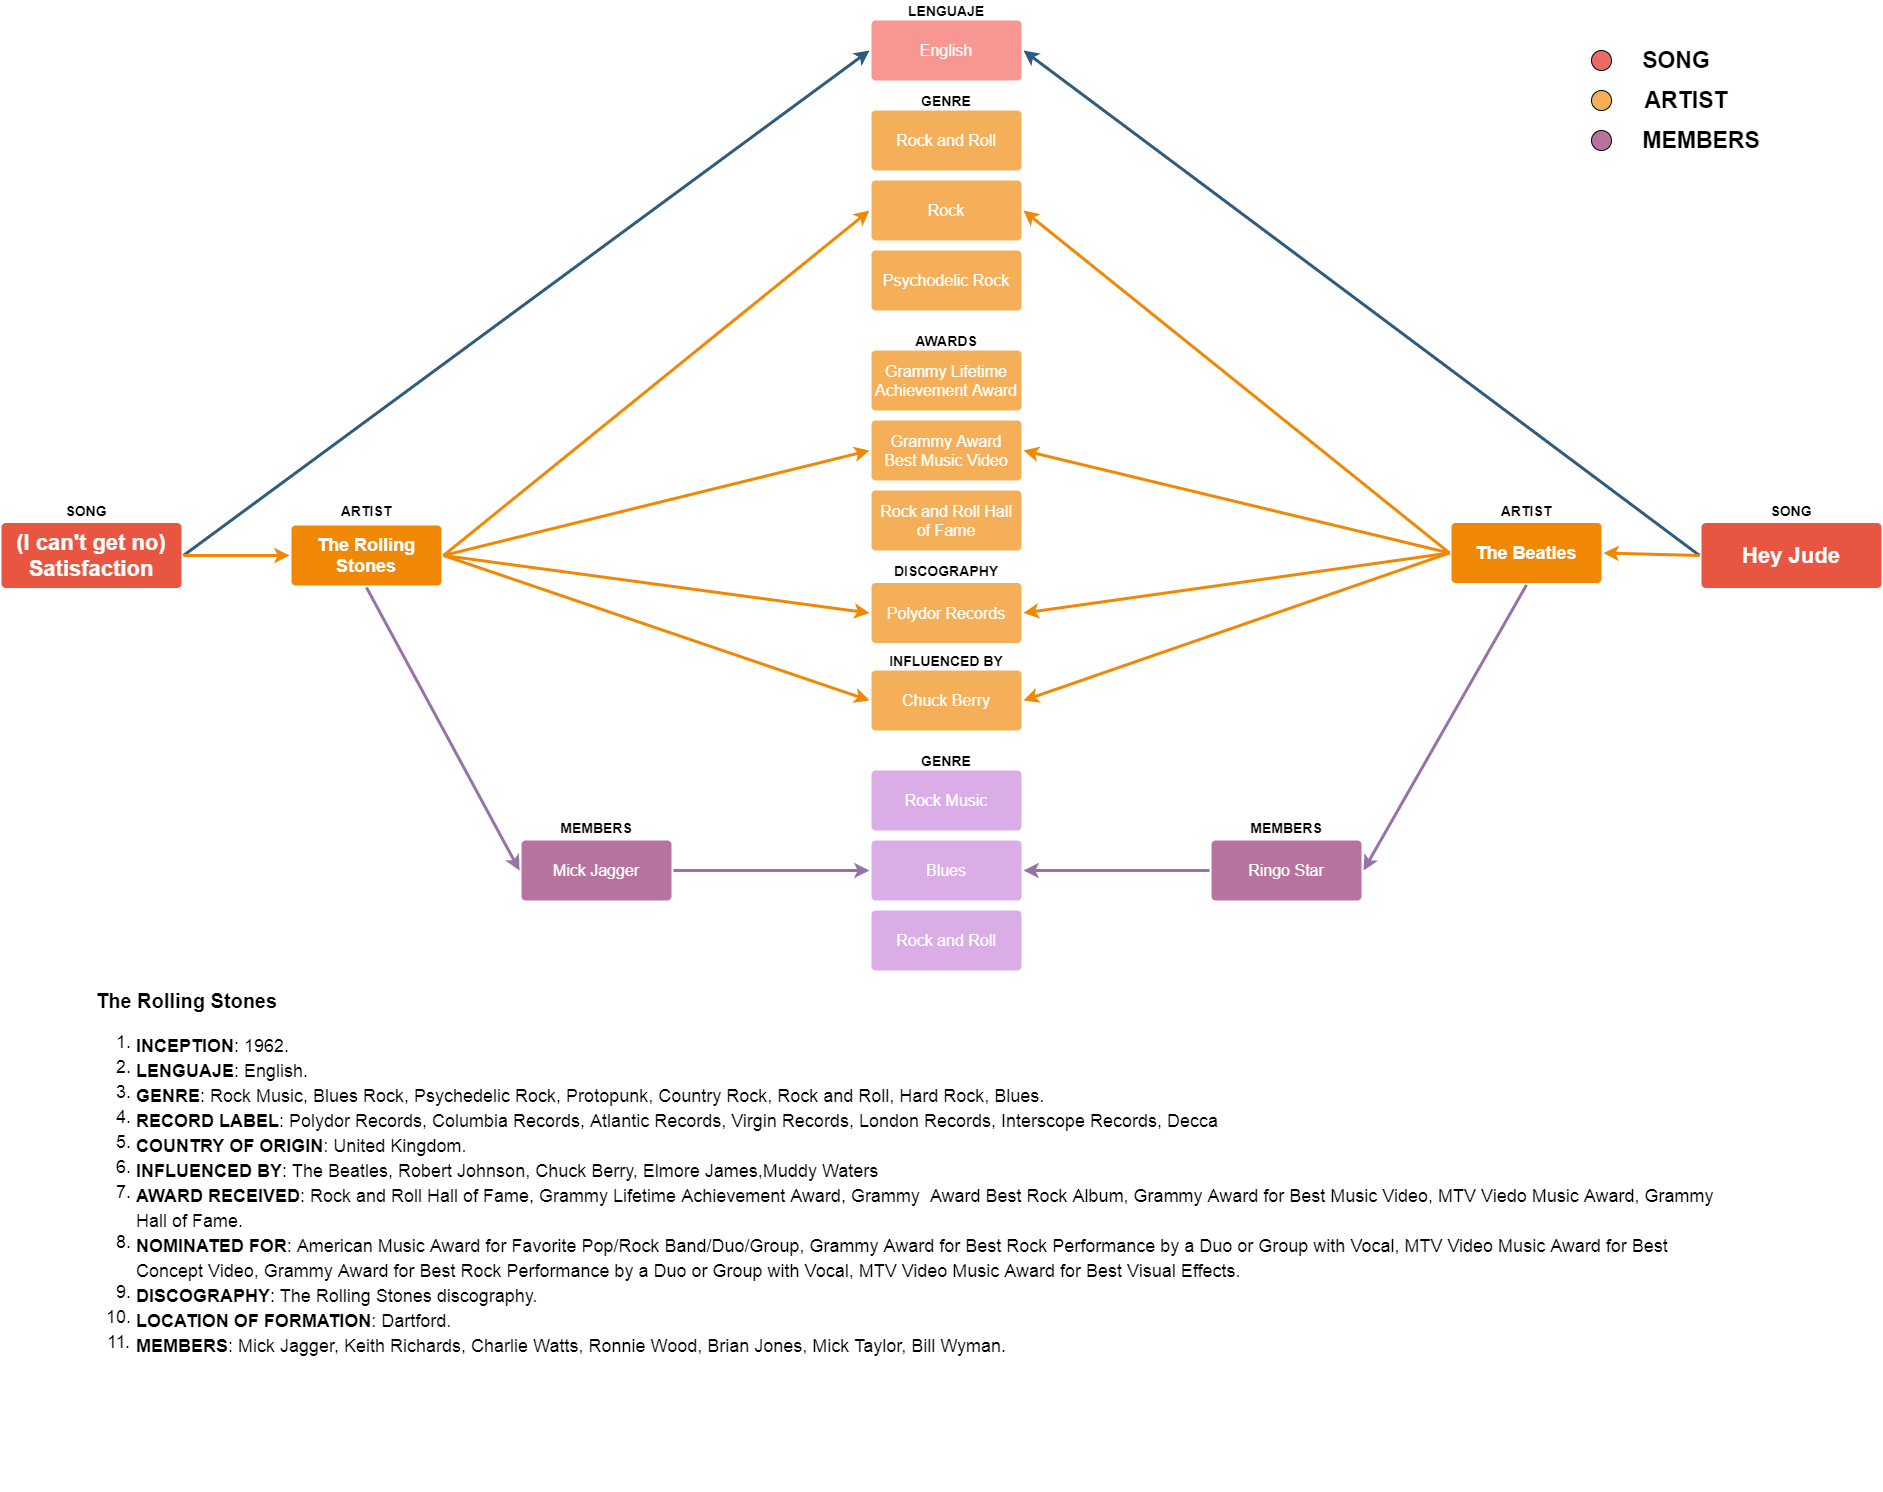
\includegraphics[width = 0.8\textwidth]{Imagenes/Bitmap/InterfaceResult.png}
	\caption{Primer diseño de la interfaz web}
	\label{fig:sampleImage}
\end{figure}

Es importante que la interfaz sea fácil de entender y usar, así que siempre trataremos de mantenerla lo más sencilla posible. La base de nuestro diseño es el grafo de explicaciones ya mencionado, pues es el elemento más importante debido a la gran cantidad de información que aporta y, por lo tanto, es también la parte central de la interfaz alrededor de la cual se posicionarán el resto de elementos.\\

En la Figura 1 se puede observar la primera iteración de nuestro diseño. En ella se ve un ejemplo de grafo donde los nodos son los distintos sujetos y objetos (según el modelo RDF) mientras que las aristas representan los predicados que relacionan a esos nodos.\\

Los nodos posicionados a ambos extremos son las canciones sobre las que estamos realizando el estudio, diferenciados por el color rojo. A partir de ellas parten todas las explicaciones. En el centro se puede ver también un nodo coloreado de un rojo más suave, este representa al objeto de una explicación directa (en este caso la explicación ``Idioma'').